\documentclass{bioinfo}
\copyrightyear{2005}
\pubyear{2005}

% - - - - - - - - - - - - - - - - - - - - - - - - - - - - - - - - 
% User-specific packages
% - - - - - - - - - - - - - - - - - - - - - - - - - - - - - - - - 
\usepackage{amsmath} 
\usepackage{amsfonts} 
\usepackage{xspace}
\usepackage{bm} \bm{}
\usepackage{graphicx}
\usepackage{timestamp} 

\graphicspath{{figures/col/}}

% - - - - - - - - - - - - - - - - - - - - - - - - - - - - - - - - 
% User-specific macros
% - - - - - - - - - - - - - - - - - - - - - - - - - - - - - - - - 
\newcommand{\GWS}{GWS\xspace}
\newcommand{\GWSFive}{GWS5\xspace}
\newcommand{\GWSSix}{GWS6\xspace}
\newcommand{\GWSFivef}{GenomeWideSNP\_5\xspace}
\newcommand{\GWSSixf}{GenomeWideSNP\_6\xspace}

\newcommand{\PMA}{\ensuremath{\textnormal{PM}_\textnormal{A}}\xspace}
\newcommand{\PMB}{\ensuremath{\textnormal{PM}_\textnormal{B}}\xspace}
\newcommand{\TP}{\ensuremath{\textnormal{TP}}\xspace}
%\newcommand{\TPrate}{TP rate\xspace}
%\newcommand{\TPrates}{TP rates\xspace}
%\newcommand{\FPrate}{FP rate\xspace}
%\newcommand{\FPrates}{FP rates\xspace}
\newcommand{\TPrate}{true-positive rate\xspace}
\newcommand{\TPrates}{true-positive rates\xspace}
\newcommand{\FPrate}{false-positive rate\xspace}
\newcommand{\FPrates}{false-positive rates\xspace}
% MathOperator!
\newcommand{\MAD}{\ensuremath{\textnormal{MAD}}\xspace}

\newcommand{\chrX}{ChrX\xspace}
\newcommand{\chrY}{ChrY\xspace}
\newcommand{\NspI}{\emph{Nsp}I\xspace}
\newcommand{\StyI}{\emph{Sty}I\xspace}
\newcommand{\Nsp}{\ensuremath{\textnormal{Nsp}}\xspace}
\newcommand{\Sty}{\ensuremath{\textnormal{Sty}}\xspace}

\newcommand{\filename}[1]{\textit{#1}\xspace}
%\newcommand{\url}[1]{\href{#1}{#1}\xspace}
\newcommand{\pkg}[1]{\textit{#1}\xspace}
\newcommand{\args}[1]{\textit{#1}\xspace}
\newcommand{\FL}{\textnormal{FL}\xspace}
\newcommand{\GC}{\textnormal{GC}\xspace}
\newcommand{\CN}{CN\xspace}
\newcommand{\kb}{\textnormal{kb}\xspace}
\newcommand{\bx}{\mathbf{x}\xspace}
\newcommand{\by}{\mathbf{y}\xspace}
\newcommand{\bz}{\mathbf{z}\xspace}
\newcommand{\ba}{\mathbf{a}\xspace}
\newcommand{\bb}{\mathbf{b}\xspace}
\newcommand{\bA}{\mathbf{A}\xspace}
\newcommand{\bB}{\mathbf{B}\xspace}
\newcommand{\bC}{\mathbf{C}\xspace}
\newcommand{\bS}{\mathbf{S}\xspace}
\newcommand{\bU}{\mathbf{U}\xspace}
\newcommand{\bV}{\mathbf{V}\xspace}
\newcommand{\bW}{\mathbf{W}\xspace}
\newcommand{\beps}{\bm{\varepsilon}\xspace}
\newcommand{\bnu}{\bm{\nu}\xspace}
\renewcommand{\Re}{\mathbb{R}\xspace}
\newcommand{\II}{\mathbb{I}\xspace}
\DeclareMathOperator{\median}{\textnormal{median}}
\DeclareMathOperator{\mad}{\textnormal{mad}}


%\newcommand{\citet}[1]{\cite{#1}} 
%\newcommand{\citep}[1]{\cite{#1}} 

% - - - - - - - - - - - - - - - - - - - - - - - - - - - - - - - - -
% Macros for highlighting updates
% - - - - - - - - - - - - - - - - - - - - - - - - - - - - - - - - -
\usepackage{endnotes} 
\usepackage{color} 
\definecolor{MyDarkBlue}{rgb}{0,0.08,0.45}
\definecolor{MyDarkRed}{rgb}{0.85,0.08,0}
\newcommand{\updated}[3][MyDarkRed]{{{\color{#1}\textsl{#2}}\endnote{#3 \color{#1}\textsl{#2}}}\xspace}
%\newcommand{\updated}[3][MyDarkBlue]{{{\color{#1}\textsl{#2}}}\xspace}
%\newcommand{\updated}[3][red]{{{\color{#1}\textsl{\textbf{#2}}}\endnote{#3 \textsl{#2}}}\xspace}
%\newcommand{\updated}[3][red]{{{\color{#1}\textsl{\textbf{#2}}}}\xspace}
%\renewcommand{\updated}[3][red]{#2\xspace} 



\begin{document}
\firstpage{1}

\title[CRMA~v2]{A single-array preprocessing method for estimating full-resolution raw copy numbers from all Affymetrix genotyping arrays including GenomeWideSNP 5 \& 6}
\author[Bengtsson \& Speed]{Henrik Bengtsson\,$^{\rm a}$\footnote{To whom correspondence should be addressed}, Pratyaksha Wirapati\,$^{\rm b}$, Terence P. Speed\,$^{\rm a,c}$}
\address{
  $^{\rm a}$ Department of Statistics, University of California, Berkeley, USA.
  $^{\rm b}$ Bioinformatics Core Facility, Swiss Institute of Bioinformatics, Lausanne, Switzerland.
  $^{\rm c}$ Bioinformatics Division, Walter \& Eliza Hall Institute of Medical Research, Parkville, Australia.
} 

\history{Version: \timestamp; Received on November 4, 2008; revised on April 12, 2009; accepted on XXXXX}

\editor{Associate Editor: John Quackenbush}

\maketitle

\begin{abstract}

\section{Motivation:}
High-resolution copy-number (CN) analysis have in recent years gained much attention, not only for the purpose of identifying CN aberrations associated with a certain phenotype but also for identifying CN polymorphisms.  In order for such studies to be successful and cost effective, the statistical methods have to be optimized.  We propose a single-array preprocessing method for estimating full-resolution total CNs.  It is applicable to all Affymetrix genotyping arrays, including the recent ones that also contain non-polymorphic probes.  A reference signal is only needed at the last step when calculating relative CNs.

\section{Results:}
As with our method for earlier generations of arrays, this one controls for allelic crosstalk, probe affinities and PCR fragment-length effects. Additionally, it also corrects for probe-sequence effects and co-hybridization of fragments digested by multiple enzymes that takes place on the latest chips.  
\updated{We compare our method with Affymetrix' CN5 method and the dChip method by assessing how well they differentiate between various CN states at the full resolution and various amounts of smoothing.  Although the others use data from all arrays for their preprocessing, we observe that CRMA~v2 performs as well as or better even if it is a single-array method.}{REMOVED: Using sex-chromosome HapMap data, we compare our method with Affymetrix' CN5 method and the dChip method, by assessing how well they differentiate between zero (CN=0), one (CN=1) and two (CN=2) copies at the full resolution and various amounts of smoothing.  Although the others use data from all arrays for their preprocessing, CRMA~v2 outperforms them for separating CN=1 from CN=2, and performs as well as CN5 for separating CN=0 from CN=1. ADDED:}
This shows that it is possible to do online analysis in large-scale projects where additional arrays are introduced over time.

\section{Availability:}
A bounded-memory implementation that can process any number of arrays is available in the open-source \pkg{R} package \pkg{aroma.affymetrix}. 

\section{Contact:} 
\href{hb@stat.berkeley.edu}{hb@stat.berkeley.edu}
\end{abstract}

%%%%%%%%%%%%%%%%
%% Background %%
%%
\section{Introduction}
\label{secBackground}
Following the suite of single-nucleotide polymorphism (SNP) arrays ('10K', '100K' and '500K'), Affymetrix has released a new class of chip types referred to as GenomeWideSNP ('GWS'), which in addition to SNP units include non-polymorphic probes, also called copy-number (CN) probes.  The latter can be used to estimate the amount of target DNA at loci other than SNPs.  The \GWSFivef ('\GWSFive'), released February 2007, is targeted by Affymetrix as a genotyping assay, whereas the \GWSSixf ('\GWSSix'), released May 2007, is targeted as both a genotyping and a CN assay.

In this paper we present the CRMA~v2 method for estimating full-resolution raw total copy numbers (CNs).  It extends and improves upon CRMA~\citep{BengtssonH_etal_2008} and applies to all Affymetrix genotyping arrays including \GWS and custom arrays. Likewise, it does not require genotype calls.  
It should be emphasized that the purpose of the method is to provide better raw full-resolution estimates that increase chances for downstream methods such as segmentation methods and CN calling methods to produce better estimates.

In contrast to other methods, CRMA~v2 is a single-array method that processes each array independently of the others.  In order to achieve this, we had to overcome the challenges in adapting CRMA's multi-array steps.
The access to a single-array preprocessing method has several implications: (i) Only two hybridizations are required for paired analysis, e.g. in a single-person tumor-normal study\updated{, which is further illustrated by the results in Section~\ref{secSingleSampleEvaluation}}{ADDED:}. (ii) Each array can be preprocessed immediately after being scanned.  (iii) Arrays can be processed in parallel on different hosts/processors making it possible to decrease the processing time of a set of arrays linearly with the number of processors.  (iv) There is no need to reprocess an array when new arrays are produced, which further saves time and computational resources.   Furthermore, (v) the decision to filter out poor arrays can be made later, because a poor array will not affect the preprocessing of other arrays. %%, which is illustrated by the exclusion of sample NA12145 in this study.
More importantly, a single-array method is (vi) potentially very practical for applied medical diagnostics, because individual patients can be analyzed at once, even when they come singly rather than in batches.
%%Furthermore, the decision to filter out poor samples can be made later, because a poor sample will not affect the estimates of other arrays, which is illustrated by the exclusion of sample NA12145 in this study.


The outline of this paper is as follows. 
In Methods, we start by describing important differences between the new \GWS arrays and the former SNP arrays.  
In light of this, we explain how the original CRMA model is adapted for \GWS, and how it is further enhanced by introducing a normalization step controlling for probe-sequence effects.  
Each step is modified so that it can be applied to an array independently of the others.
At the end of this section the evaluation method used for comparing with existing methods is described.
In Results, we compare the different methods based on their performances at different levels of resolution and stratified by SNP or CN loci.
In the Discussion, we conclude the study and give future research directions.



\section{Methods}
\subsection{Overview of the \GWS arrays}

%\section*{Additional features of the \GWS arrays and assays}
The \GWSSix chip type interrogates 931,946 SNPs and 945,826 CN loci totaling 1,877,772 loci, whereas \GWSFive interrogates 500,568 SNPs and 417,269 CN loci totaling 917,837 unique loci.  \GWSFive has the same set of SNPs as the 500K chip set, whereas for \GWSSix 6,238 of those have been replaced by a new set of 437,616 SNPs.  Among CN loci, only 61,846 are identical on \GWSFive and \GWSSix.
%
In contrast to previous generation of chip types~\citep{BengtssonH_etal_2008}, there are no  mismatch but only perfect-match (PM) probes.  
On \GWSFive, all SNPs have 4 replicated (\PMA, \PMB) pairs.  On \GWSSix there are either 3 or 4 such pairs. These probe pairs are identical replicates, whereas before they were slightly shifted relative to the SNP position.
%
For both \GWS arrays, the pairs in each SNP were selected such that they optimized the genotype performance.  For the \GWSFive there was no constraint that the \PMA and \PMB sequences had to be aligned on the genome, causing 192,399 (38.4\%) SNPs to have misaligned \PMA and \PMB.  There was also no constraint that \PMA and \PMB should be on the same strand, resulting in 46,176 (9.22\%) SNPs with \PMA and \PMB on opposite strands.  These constraints were reintroduced for \GWSSix.
More details on the \GWS arrays are available in the Supplementary Notes.

%%\subsection*{Co-hybridization of fragments digested by multiple enzymes}
%% \label{secMultiEnzymeDigestion}
For the 100K as well as the 500K SNP-only assays, DNA is prepared in two parallel processes, each digesting the DNA using a unique enzyme, amplifying the fragments by PCR, and hybridizing the products to separate arrays.  In the GWS assays, which like 500K, uses enzymes \NspI and \StyI, the two mixes of PCR products are no longer hybridized to separate arrays but instead to the same array~\citep{Affymetrix_2007f, Affymetrix_2007g}.
Consequently, some of the SNP target DNA of PCR products originating from different restriction digestions (enzymes) will hybridize to the same probe.  
The non-polymorphic (CN) probes were designed to target DNA either from both enzymes or \NspI exclusively, but not from \StyI alone.  
For an explanation of this and a summary of how many SNP and CN loci are targeted by the two enzymes, see the Supplementary Notes.
%% This has to be accounted for in  when, for instance, fitting the fragment-length normalization.


Finally, for \GWSFive and \GWSSix, Affymetrix has identified 59,744 (6.51\% of all loci) and 25,346 (1.35\%) SNPs, respectively, that do not meet their quality criteria (private communication).
In order to differentiate between the filtered and non-filtered sets of loci, Affymetrix provides one ``default'' chip definition file (CDF) and one ``full'' CDF.  Further details on the two types of CDFs is given in the Supplementary Notes.



%%%%%%%%%%%%%%%%%%
%\section{Methods}
%\label{secMethods}



%--------------------------------------------------------------------------
% PROPOSED MODEL
%--------------------------------------------------------------------------
\subsection{Proposed model}

The CRMA~v2 method takes an approach similar to CRMA~\citep{BengtssonH_etal_2008} for estimating total (non-polymorphic) CNs.  The model for allelic-crosstalk calibration is adapted to \GWS, because of the added non-polymorphic probes.  After this calibration, we utilize a nucleotide-position model~\citep{CarvalhoB_etal_2007} to normalize for small difference across arrays but also for allelic imbalances in \PMA and \PMB.  
In contrast to our previous multi-array model, we here use a single-array model to summarize the probes.  At the end, PCR fragment-length normalization is updated to model the multi-enzyme hybridization.
%%
CRMA~v2 was designed to be:
(i) backward compatible with previous generations of arrays,
(ii) prepared for future generations of arrays, 
(iii) sequential, so that it is easy to replace or add other steps, and
(iv) such that each array can be processed independently of the others.
The latter allows for online single-array CN analysis, which becomes more important as larger data sets are being generated and updated over time, as well as it allows for analyzing very small data sets.
It is only in the last step while calculating \emph{relative} CNs that a reference is needed.
Although not discussed further in this paper, we also look toward a unified method for estimating allele-specific CNs.


\subsubsection{Calibration for offset and crosstalk between alleles}
\label{secModelACC}
For reasons explained in \citet{BengtssonH_etal_2008}, the (\PMA,\PMB) signals are affected by allelic crosstalk.  It was shown that correcting for crosstalk as well as offset significantly improved the ability to differentiate between CN states.
The offset \& crosstalk model introduced in \citet{BengtssonH_etal_2008} needs to be modified for \GWS arrays in order to control for offset in the new non-polymorphic probes.  
%% Similarily, for the subset of SNPs on \GWSFive that have the two alleles on opposite strands we do not expect crosstalk but we still need to correct for offset.
%%
For SNPs, let $\bx_{ijk} = (x_{ijkA}, x_{ijkB})$ and $\by_{ijk} = (y_{ijkA}, y_{ijkB})$ denote the true and the observed signals for probe pair $(j,k)$ in SNP $j$, probe $k=1,\ldots,K_j$, and sample $i=1,\ldots,I$.  
Without loss of generality, assume that probes in each pair are ordered lexicographically by the SNP nucleotides, resulting in six possible pairs.  For a particular pair, we model the allelic crosstalk and shift observed in $\{\by_{ijk}\}$ by an array-specific affine transformation as
\begin{equation}
  \by_{ijk} = \ba_i + \bS_i \bx_{ijk} + \beps_{ijk},
  \label{eqnACCi}
\end{equation}
where $\ba_i = (a_{iA}, a_{iB})^T$ denotes the offset, 
\begin{equation}
 \bS_i = 
 \begin{bmatrix}
   S_{iAA} & S_{iAB} \\
   S_{iBA} & S_{iBB}
 \end{bmatrix}
  \label{eqnACCii}
\end{equation}
is the crosstalk matrix, and $\beps_{ijk} = (\varepsilon_{ijkA}, \varepsilon_{ijkB})^T$ is noise.  The affine parameters in this model are estimated based on the subset $\mathcal{J^*}$ of loci that are likely to be copy neutral regardless of sample, i.e. ChrX and ChrY data are excluded.  If some of the remaining loci are not copy neutral, we rely on robustness of the estimator to get unbiased estimates.
Estimates of the true signals
%% (up to a multiplicative constant) 
are obtained by backtransforming as
\begin{equation}
  \hat{\bx}_{ijk} = \hat{\bS}^{-1}_i (\by_{ijk} - \hat{\ba}_i).
  \label{eqnACCiii}
\end{equation}
\updated{In words, the crosstalk correction for SNPs is performed by treating the data as points sampled from a polyhedral cone in multidimensional space. The apex ($\ba_i$) of the cone is the baseline intensity for all channels, and edges (defined by $\bS_i$) are directions corresponding to pure signals.  Zeroing the apex and orthogonalizing the edges remove the baseline and the crosstalk. The cone is fitted iteratively by minimizing the distance from the cone to the points that lie outside it \citep{WirapatiSpeed_2002}.}{REMOVED: For further details, see~\citet{BengtssonH_etal_2008}. ADDED:}
For other non-SNP probes, including CN probes, we estimate and correct for the offset as the weighted average of offsets across all six nucleotide pairs with weights inversely proportional to the number of data points in each group.  The reason for calculating the offset this way is the belief that there is a dominant offset that is shared by all probes, e.g. scanner offsets~\citep{BengtssonH_etal_2004}, \updated{a view which is}{REMOVED: which is further ADDED:} strengthened by our parallel studies on Affymetrix resequencing arrays.  This \updated{would also suggest}{REMOVED: This also suggests ADDED:} that the offsets in Eqn~\eqref{eqnACCi} should be symmetric in the two alleles and same for all six pairs, but for practical reasons~\citep{BengtssonH_etal_2008} we \updated{do}{REMOVED: choose: ADDED:} not do this.

Another difference from CRMA~(v1) is that after correcting for offset, all probe signals are rescaled to have the same arbitrary average $(=2200)$.  In \citet{BengtssonH_etal_2008} this was done for each nucleotide pair separately, but if done \updated{here}{ADDED:} introduces systematic biases between SNPs and CN loci due to enzymatic mixture imbalances.

\subsubsection{Normalization for probe-sequence effects}
\label{secModelBPN}
It has been shown that the affinity of a probe can be attributed to its sequence composition~\citep{BinderH_etal_2004a, ZhangL_etal_2007, CarvalhoB_etal_2007}.
As in \citet{CarvalhoB_etal_2007}, we model the probe-sequence affinity as a function of nucleotide and position in order to control for (i) small fluctuations in probe affinities across arrays, and (ii) differences in \PMA and \PMB affinities. 
Consider all probes $k'=1,\ldots,K'$ on the array and let $\bb_{k'} = (b_{k',1},b_{k',2},\ldots,b_{k',25})$ be the probe sequence for probe $k'$ with nucleotide $b_{k',t} \in \{A,C,G,T\}$ at position $t=1,\ldots,25$.
According to the probe-position model~\citep{CarvalhoB_etal_2007}, the crosstalk and offset calibrated signals $\hat{x}_{ik'}$ for probe $k'$ of a given array $i=1,\ldots,I$, can be described (on the intensity scale) by:
\begin{equation}
  \hat{x}_{ik'} = \rho_{ik'} \cdot \mu_{ik'} + \xi_{ik'},
  \label{eqnBPNi}
\end{equation}
where $\mu_{ik'}$ is the overall mean signal, $\rho_{ik'} > 0$ is the array and sequence-specific affinity, and $\xi_{ik'}$ is noise.  The affinities are modeled on the logarithmic scale as:
\begin{equation}
  \log_2 \rho_{ik'} = \log_2 \rho_{i}(\bb_{k'}) 
    = \sum_{b \in \{A,C,G,T\}} \sum_{t=1}^{25} \II(b_{k',t}=b)h_{i,b}(t),
  \label{eqnBPNii}
\end{equation}
where $\{h_{i,b}(\cdot)\}_b$ are nucleotide-specific smooth functions and $\II(\cdot)$ is the indicator function.  The model is constrained such that $\sum_{b \in \{A,C,G,T\}} h_{i,b}(t) = 0$ at each position $t$.
We choose to model $\{h_{i,b}(\cdot)\}_b$ with cubic splines with 5 degrees of freedom (we get very similar results for 7 and 9 d.f.).  The model is fitted on the logarithmic scale with non-positive signals excluded, and as before, only to the subset of probes that are expected to be copy neutral.
Given estimates $\{\hat{h}_{i,b}(\cdot)\}_b$, \emph{all} probe signals can be normalized as:
\begin{align}
  \tilde{y}_{ik'} &= \hat{x}_{ik'} / \hat{\rho}_{i}(\bb_{k'}),
  \label{eqnBPNiii}
\end{align}
where $\{\tilde{y}_{ik'}\}$ denotes the offset \& crosstalk calibrated and probe-sequence normalized signals. %% and $\{\hat{\rho}_{ik'}\}$ are calculated as in Eqn~\eqref{eqnBPNii} with estimates plugged in.
%% Because Eqn~\eqref{eqnBPNi} is on the logarithmic scale and the crosstalk calibration introduce non-positive signals, we shift the signals $e$ (=300) units in order to decrease the number of non-defined values, cf.~\citet{BengtssonH_etal_2008}.
As in \citet{CarvalhoB_etal_2007}, we observe small systematic effects across arrays $\{h_{i,b}(\cdot)\}_b$, which introduce extra variance.  In addition, the difference in affinity between \PMB and \PMA is $h_{i,b_B}(t) - h_{i,b_A}(t)$ where $t$ is the SNP probe position.  If not controlled for, it will bias heterozygote signals (AB) relative to homozygote signals (AA or BB), when calculating the total signals.
We note that the latter effect can be controlled for by introducing a heterozygote component in the crosstalk model, but as argued in~\citet{BengtssonH_etal_2008} such an approach is likely to be sensitive to model errors, e.g. when there are a lot of CN aberrations which may be the case for some tumors.


\subsubsection{Probe-level summarization}
\label{secSummarizationModel}
With technically replicated probes, \updated{as in the most recent chip types \GWSFive and \GWSSix}{ADDED:}, and assuming that the effect from neighboring probes is negligible, probe affinities used in multi-array summarization models~\citep{BengtssonH_etal_2008} will vanish.
%%  Also, in contrast to previous chip types, where $(\PMA,\PMB)$ pairs were shifted relative to the SNP location, there is no unique pairing of \GWS replicated probes.
%% Moreover, pairing probes based on such a rule, would require not only that this is true for all probes but also a tedious verification of the spatial location of each probe for existing and future chip types.
For these reasons, we consider the following single-array summarization estimates for total CNs:
\begin{align}
%%  \hat{\theta}_{ijA} &= \median_{k} \{\tilde{y}_{ijkA}\}, \notag \\
%%  \hat{\theta}_{ijB} &= \median_{k} \{\tilde{y}_{ijkB}\}, \notag \\
%%  \hat{\theta}_{ij}  &= \hat{\theta}_{ijA} + \hat{\theta}_{ijB},
  \tilde{y}_{ijk} &= \tilde{y}_{ijkA} + \tilde{y}_{ijkB}, \notag \\
  \hat{\theta}_{ij} &= \median_{k} \{\tilde{y}_{ijk}\},
  \label{eqnSumAllele}
\end{align}
where the median is calculated across all probe-pair sums $k=1,\ldots,K_j$ in SNP $j$.
%% Note, there is nothing in Model~\eqref{eqnSumAllele} that requires equal number of allele~A and allele~B probes.
\updated{For older chip types (10-500K) for which the replicated probes are slightly shifted along the genome, it is still sensible to model the probe affinities using a multi-array model such as the log-additive model used in \citet{BengtssonH_etal_2008}.  Since these chip types are considered outdated, we have not conducted a formal study comparing the two summarization models, but from our experience we do note a small gain when using the log-additive model (no such gain is observed for \GWSSix). Thus, for these arrays, the choice will be a trade off of receiving this gain and having the option to process each array independently of the others.}{ADDED:}

Finally, for non-polymorphic loci, which are all single-probe units (as defined by the CDFs used here), we let
\begin{equation}
  \hat{\theta}_{ij} = \tilde{y}_{ij1}
  \label{eqnCnAB}
\end{equation}
be the corresponding estimates for unit/probe $j$ in sample $i$.  If in future chip types, or related custom genotyping arrays, there are replicated non-polymorphic probes, Eqn~\eqref{eqnCnAB} should be replaced by summaries as in Eqn~\eqref{eqnSumAllele}.  

%% In \citet{BengtssonH_etal_2008}, we utilized a log-additive multi-array model for total copy numbers that controls for differencies in affinities of probes  part of the same SNP.  For a given SNP $j$, the normalized probe signals $\{(\tilde{y}_{ijkA},\tilde{y}_{ijkB})\}_{ik}$ are modelled as:
%% \begin{align}
%%   \tilde{y}_{ijk} &= \tilde{y}_{ijkA} + \tilde{y}_{ijkB}, \notag \\ 
%%   \log_2{(\tilde{y}_{ijk}+e)} &= \log_2\theta_{ij} + \log_2\phi_{jk} + \xi_{ijk},
%%   \label{eqnPLM}
%% \end{align}
%% where $\{\theta_{ij}\}_i$ are the chip effects, $\{\phi_{jk}\}_k$ are the probe affinities, and $\{\xi_{ijk}\}_{ik}$ is noise.  As before, we utilize an artifical shift $e$ (=300) because of the logarithmic transform.  For further details, see \citet{BengtssonH_etal_2008}. 




%% We note that the allele-specific estimates in Eqn~\eqref{eqnSumAllele} are remotely comparable to the 'Avg Diff' score used in MAS~4.0 for gene expression analysis, where a robust average is calculated across a selected set of perfect match (PM)/mismatch (MM) probe-pair differences~\citep{Affymetrix_2001}.  They are also comparable to the non-robust average [sum?] used in the CNAG method~\citep{NannyaY_etal_2005} for 100K and 500K copy-number analysis.
%% Finally, we would like to emphasize that Eqns~\eqref{eqnSumAllele}-\eqref{eqnSumSnpAB} constitute a single-chip summarization method, that is, it can be applied to each array separately.  Thus, in contrast with the multi-chip model in Eqn~\eqref{eqnPLM}, it is possible to summarize probe signals 'online' as new arrays arrive.




\subsubsection{Normalization for fragment-length effects}
\label{secFLnorm}
%% We have found that it is important that the preprocessing models takes this multi-enzyme digestion into account, otherwise there is a substantial risk for getting systematic biases between SNPs and CN loci due to enzymatic mixing imbalances.
%% [We will later see that the hybridization of two PCR products on the same array requires a special model in order to control for confounded effects due to mixing inbalances.]
%% As with the Affymetrix 500K assay, in the GWS assays DNA is digested using two different restriction enzymes (\NspI and \StyI).  The difference is that, after ligating with corresponding adaptors and PCR amplification, the PCR products are in latter assays combined, purified, post-fragmented, labeled and hybridized together to the same array. 
Because fragments from two enzymes are hybridized to the same array for \GWS, some probes will match fragments originating from both restriction digestions.  See the Supplementary Notes for details on how many SNP and CN loci are exclusively on \NspI, on \StyI, and on both.
%% For the \GWSSix chip type, out of the 931,306 SNPs, 523,573 (56.2\%) are on both fragments, 246,514 (26.5\%) only on NspI, and 161,219 (17.3\%) only StyI.  For the 945,806 CN loci, there are 494,615 (52.3\%) on both, 451,191 (47.7\%) on NspI alone, but none on StyI alone.
For signals originating from only one of the digestions, we could, for each enzyme separately, apply the fragment-length normalization method proposed in \citet{BengtssonH_etal_2008}.  However, because a signal that originates from both digestions consists of one \NspI and one \StyI component, which each has been amplified differently, another method has to be used for such units.  For this reason, we modify the method in \citet{BengtssonH_etal_2008} as described next. 

First, assume that the number of fragments obtained from digesting with a particular enzyme is independent of locus $j$.  This assumption was implicit in \citet{BengtssonH_etal_2008}.
%% We recognize that an enzyme might produce fragments in different proportions due to differences in recognition or adaptor sequences~\citet{Affymetrix_2007m}, but since we have found that it does not improve CRMA~v2.
Continuing, let $\lambda^{r}_j$ be the length of the fragment that was digested by restriction enzyme $r \in \{\Nsp, \Sty\}$ and contains locus $j$.
%% These lengths are predetermined by the restriction sites of the enzymes.
For sample $i=1,\ldots,I$, assume that the amount of PCR amplification of a fragment from digestion with enzyme $r \in \{\Nsp, \Sty\}$ is proportional to $2^{h^{r}_{i}(\lambda^{r}_{j})}$, where $h^{r}_{i}(\cdot)$ is a sample-specific smooth function on the logarithmic scale.
%%  We note that there is nothing per se that makes $h^{r}_{i}(\cdot)$ differ between enzymes.  However, mainly because it is easier to control for non-aliquot mixing of PCR products, we choose to model the effect separately for the two enzymes.
Next, labeled PCR products of the two digestions are mixed together.  Let $\rho^{r}_{i} > 0$ be the total amount of product for enzyme $r$ in sample $i$ \emph{relative to the \NspI enzyme}, such that $\rho^{\Nsp}_{i}=1$ for all samples.
Furthermore, assume that the amount of target hybridized to a specific probe is proportional to the number of labeled sequences.  When targets from more than one digestion (enzyme) hybridize to the same probe, assume there is no preference for either enzyme. 
Next, let $\kappa_{i} > 0$ be the overall efficiency of hybridization, scanning, image analysis etc. for array $i$ \emph{relative to the first array}, such that $\kappa_{1} = 1$.
Finally, define $g^{r}_{i}(\cdot)$ such that $2^{g^{r}_{i}(\lambda^{r}_{j})} = \kappa_{i} \rho^{r}_{i} 2^{h^{r}_{i}(\lambda^{r}_{j})}$ describes, as a scale factor, the overall systematic effect for locus $j$ in sample $i$  due to fragmentation, PCR amplification, mixing, hybridization and so on.
To conclude, for a probe interrogating sequences from both digestions, we assume that the signal for sample $i$ at locus $j$ is proportional to:
 \begin{equation}
  2^{g^{\Nsp}_{i}(\lambda^{\Nsp}_{j})} + 2^{g^{\Sty}_{i}(\lambda^{\Sty}_{j})}
  = \kappa_{i} \left(
      2^{h^{\Nsp}_{i}(\lambda^{\Nsp}_{j})}
      + \rho^{\Sty}_{i} 2^{h^{\Sty}_{i}(\lambda^{\Sty}_{j})}
    \right)
 \end{equation}
We say that \emph{the confounded fragment-length effect is additive on the intensity scale}. %% (for loci occuring on both enzymes).
%%  With everything else the same, assuming aliquot mixing proportions and ignoring other scale factors, then $n_{j} \cdot [ 2^{g^{\Nsp}(\lambda^{\Nsp}_{j})} + 2^{g^{\Sty}(\lambda^{\Sty}_{j})} ]$ copies are hybridized to the array.
With this model, each fragment-length effect $\{g_i^r(\cdot)\}_r$ can be estimated from signals exclusively from a single digestion.

In \citet{BengtssonH_etal_2008} we normalized the data toward target fragment-length effects estimated as the average effects across arrays.  
%% Without loss, this keeps the common effects such that it is possible to apply additional fragment-length models downstreams. However, 
In the effort to avoid multi-array estimators in CRMA~v2, we here normalize data toward fixed target effects.  
The choice of target functions is not important because the effects will cancel out when CN ratios relative to a reference is calculated.
Using the notation of \citet{BengtssonH_etal_2008}, we use constant target functions $g_T^r(\lambda) = \log_2(2200)$, where $2200$ was chosen arbitrary.

Define $\mathcal{J}^{\Nsp}, \mathcal{J}^{\Sty}, \mathcal{J}^{\Nsp\cap\Sty} \subset \mathcal{J}$ to be the subsets of loci that are exclusive to \NspI, \StyI, and to both enzymes, respectively.
In order to simplify the notation, we will use the same notation for the true and the estimated functions.  The normalization algorithm for array $i=1,\ldots,I$ is then:
\begin{enumerate}
 \item[1.] For each enzyme $r \in \{\Nsp, \Sty\}$, fit a smooth spline $g^{r}_{i}(\cdot)$ robustly to $\{(\lambda^{r}_{j}, \log_2\theta_{ij})\}$ based on copy-neutral loci $j \in \mathcal{J}^{r} \cap \mathcal{J^*}$ that are exclusive to restriction enzyme $r$.  This constitutes the \emph{fragment-length effect for enzyme $r$ in sample $i$}.

 \item[2.] For each enzyme $r \in \{\Nsp, \Sty\}$, calculate the \emph{PCR discrepancies for sample $i$} based on \emph{all loci} $j \in \mathcal{J}^{r}$ that are exclusive to restriction enzyme $r$ as
  \begin{equation}
    \log_2 \hat{\delta}_{ij} 
     = g^{r}_{i}(\lambda^{r}_{j}) - g^{r}_{T}(\lambda^{r}_{j})
    \label{eqnPCRbias}
  \end{equation}

 \item[3.] For remaining loci $j \in \mathcal{J}^{\Nsp\cap\Sty}$, calculate the discrepancies as
  \begin{equation}
    \log_2 \hat{\delta}_{ij} 
     = g^{\Nsp\cap\Sty}_{i}(\lambda^{\Nsp}_{j}, \lambda^{\Sty}_{j}) - g^{\Nsp\cap\Sty}_{T}(\lambda^{\Nsp}_{j}, \lambda^{\Sty}_{j})
    \label{eqnPCRbiasIIIa}
  \end{equation}
  where
  \begin{equation}
    g^{\Nsp\cap\Sty}_{i}(\lambda^{\Nsp}, \lambda^{\Sty}) = \log_2\left[
      2^{g^{\Nsp}_{i}(\lambda^{\Nsp})} + 2^{g^{\Sty}_{i}(\lambda^{\Sty})}
    \right],
    \label{eqnPCRbiasIIIb}
  \end{equation}
  and $g^{\Nsp\cap\Sty}_{T}(\lambda^{\Nsp}, \lambda^{\Sty})$ defined analogously.


 \item[4.] Finally, normalize all loci (on the intensity scale) by
  \begin{equation}
    \tilde{\theta}_{ij} = \hat\theta_{ij} / \hat{\delta}_{ij}.
    \label{eqnPCRnorm}
  \end{equation}
\end{enumerate}

%% Eqns~\eqref{eqnPCRbiasIIIa}-\eqref{eqnPCRbiasIIIb} are because $2^{g^{r}(\cdot)}$ corresponds to $\rho^{r}(\cdot)$ above.

%%No correction is made for loci where no annotation is available (Supplementary Notes).
Loci for which annotation is missing (Supplementary Notes) are rescaled such that their median signal equals the median of the other loci.
%% (excluding ChrX and ChrY, that is). /HB 2008-09-11
%%
For chip types such as 10K, 100K and 500K, where there are no multi-enzyme loci ($\mathcal{J}^{\Nsp\cap\Sty} = \emptyset$), Step~3 no longer applies and the method becomes effectively identical to the one presented in \citet{BengtssonH_etal_2008} (if the target effect is estimated from the average array).
%% Moreover, as long as there are enough loci that are exclusively digested by each enzyme, so that the enzyme-specific fragment-length effects can be estimated, then the above method also applies to cases where more than two enzymes are used.  See the Supplementary Notes for the number of loci exclusively on one enzyme.
%% One could argue that an weighted average based on an estimates of $\rho^{\Nsp}_{i}$ and $\rho^{\Nsp}_{R}$ should be used in Eqn~\eqref{eqnPCRbiasIIIb} in order to controlling for global imbalances between enzymes.  For instance, in the current setup, signals originating for an enzyme that are significantly lower than the other enzyme on a particular samples, will have less impact on the estimated correction factors.  
Moreover, since each $g^{r}_{i}(\cdot)$ includes the term $\rho^{r}_{i}$, the above method will also control for imperfect mixing of enzyme products, which otherwise carry through introducing systematic effects in loci that originate from both digestions.
Analogously, the scale differences between arrays, $\{\kappa_i\}$, are also controlled for.

\subsubsection{Normalization for GC-content effects}
\label{secGCnorm}
\updated{As in the \citet{BengtssonH_etal_2008} study, we did not find any significant GC-content effects remaining after applying CRMA~v2 and correcting for it did not improve the performance.  For this reason, we do not consider GC-content normalization here.
We wish to note that this does not necessarily contradict other studies that report strong GC-content effects.  The reason for this may be due to differences in the preprocessing methods, especially in how they correct for offset.}{ADDED:} 



\subsubsection{Calculation of raw copy numbers}
\label{secRawCN}
As in \citet{BengtssonH_etal_2008}, we calculate raw CNs as the chip effect relative to a reference.  This is the only step in CRMA~v2 requiring a reference.
We calculate the relative \CN for sample $i$ and locus $j$ as:
\begin{equation}
  C_{ij} = 2 \cdot \frac{\tilde\theta_{ij}}{\tilde\theta_{Rj}},
  \label{eqnCnRatio}
\end{equation}
where $\tilde\theta_{Rj}$ is the reference signal, which commonly is the robust average across samples and possibly corrected for the case that some data points are from non-copy-neutral loci, cf. \citet{BengtssonH_etal_2008}.
Note that for paired studies such as tumor-normal comparisons, the normal DNA will serve as the reference, which is why only two hybridizations are needed in such comparisons.
In Eqn~\eqref{eqnCnRatio} we assume that the mean of $\tilde\theta_{Rj}$ corresponds to $\CN=2$, e.g. ChrY reference estimates should be rescaled accordingly.
For \CN estimates on the logarithmic scale, we calculate:
\begin{equation}
  M_{ij} = \log_2 \frac{\tilde\theta_{ij}}{\tilde\theta_{Rj}}.
  \label{eqnCnLogRatio}
\end{equation}
Note that the latter is not defined for zero copy-number levels (or for negative levels occurring due to noise).


\subsubsection{Filtered and non-filtered set of loci}
Regardless of whether CN analysis will be conducted on a filtered or the full set of loci, we recommend that all preprocessing is done on the full set and filtering is applied only after obtaining raw CNs.  %% , for instance, before doing segmentation.  
The rationale for this is that we believe the main systematic effects are the same for the filtered and the full set and that one can estimate these effects more accurately using the latter.
This also has the advantage that the preprocessing will be the same regardless of which set is used in the end.


\subsection{Implementation}
The above preprocessing method, referred to as \emph{CRMA~v2}, is available as part of \pkg{aroma.affymetrix}~\citep{BengtssonH_etal_2008b} implemented in \pkg{R}~\citep{RDevel_2008}.
The method is designed and implemented to have bounded-memory usage, regardless of the number of arrays.
%% The  method is designed and implemented to have bounded-memory limits, meaning any number of arrays can be processed.
Since it is a single-array method, the arrays can be processed in parallel on multiple hosts/processors.



%--------------------------------------------------------------------------
% DATA SET
%--------------------------------------------------------------------------
\subsection{Data sets}
\updated{Two publicly available data sets were used in this study.}{ADDED:}
\textbf{Normal data set:} 
%% \textbf{\GWSSix:} 
\GWSSix CEL files for the 30 male and 30 female CEU founders of The International HapMap Project~\citep{HapMap_2003, AltshulerD_etal_2005} was used. Offspring were excluded in order to avoid biological relationships.
%% \textbf{\GWSFive:} There is no public \GWSFive data available for the above \GWSSix HapMap samples but only for a subset consisting of 20 founders with 10 children, where we choose to use the latter in order to increase the sample size. 
Because female NA12145 has a low true \chrX CN level \citep{TingJ_etal_2006}, it was excluded from the evaluation.  
\updated{
\textbf{Tumor-normal data set:} 
All 68 \GWSSix CEL files of the GEO data set GSE13372~\citep{ChiangD_etal_2009}, which among other samples contains 21 replicated tumor-normal HCC1143 (breast ductal carcinoma) pairs, were processed.  The evaluation was done on the first tumor-normal HCC1143 pair.
}{ADDED:}
More details on the \updated{above data sets}{REMOVED: data ADDED:} can be found in the Supplementary Notes.


%--------------------------------------------------------------------------
% EVALUATION METHODS
%--------------------------------------------------------------------------
\subsection{Methods for evaluation}
\label{secEvaluation}
In order to assess the performance of CRMA~v2, we compared it with Affymetrix CN5 method~\citep{Affymetrix_2008m} and the method implemented in dChip~\citep{LiWong_2001}.  For \emph{dChip}, we found that summarizing SNP probes by averaging is significantly better than using the default multiplicative model.  For this reason, we only present results for the former (here denoted by \emph{dChip*}).
%% dChip*: I have verified that the exported MBEI estimates are the same as the ones in the DCP files.  In other words, the poor SNP performance for dChip* is not due to an error in reading in exported data. /HB 2008-02-01
%%
\updated{Moreover, since the CN5 implementation is limited to the default CDF, the results presented here are based on that set of loci.}{MOVED:}
\updated{As outlined below, we base the evaluation on the aforementioned data sets using a multi-sample evaluation and a single-sample single-changepoint evaluation, respectively.  Further details are available in the Supplementary Notes.}{ADDED:}

\subsubsection{Multi-sample ChrX \& ChrY evaluation}
\updated{For the normal data set,}{ADDED:} we used the same set of \updated{Receiver Operator Characteristics (ROC)}{ADDED:} evaluation methods as in \citet{BengtssonH_etal_2008} using relative (Eqn~\eqref{eqnCnRatio}) instead of log-ratio CNs (Eqn~\eqref{eqnCnLogRatio}).
To assess how well the methods differentiate between one and two copies, and zero and one copy, we use ChrX and ChrY data, respectively.  We exclude loci in pseudo-autosomal regions~\citep{BlaschkeRappold_2006} and inside and close to known CN polymorphic regions~\citep{RedonR_etal_2006}\updated{, leaving 68,966 ChrX loci and 5,718 ChrY loci.}{ADDED:}
%%
Since CN5 uses only females (males) for the reference signals $\{\tilde\theta_{Rj}\}$ on ChrX (ChrY), this comparison study will not use bias-corrected reference signals from all samples \citep{BengtssonH_etal_2008}.

\subsubsection{Single-sample evaluation at a set of changepoints}
\updated{For the tumor-normal data set, we selected one tumor-normal pair for which we identified a set of regions each containing a single CN change point.
Data points in a 500kb region centered around each change point were excluded.  The remaining data points are annotated to belong to either the copy-neutral state or the copy-aberrant state.  Contrary to the evaluation on the normal data set, the true CN levels are not known except that they are either gains or losses.
Next, for each CN region we use ROC analysis to assess how well the raw CNs separate between the neutral and the aberrant data points.  This evaluation is done on the full-resolution CNs as well as smoothed CNs, where the CNs are smoothed by using non-overlapping bins for which the average CNs is calculated.
This approach was inspired by studies such as \citet{LaiW_etal_2005}, and \citet{WillenbrockFridlyand_2005}.}{ADDED:}



 
%%%%%%%%%%%%%%%%%%%%%%%%%%%%
%% Results and Discussion %%
%%
\section{Results}
\label{secResults}

\subsection{Multi-sample evaluation}

\subsubsection{Differentiating CN=1 and CN=2 (ChrX)}
\updated{As explained in detail in \citet{BengtssonH_etal_2008}, we use ChrX data to assess how well a set of CN estimates can differentiate between the CN=2 (females) state and the CN=1 (males) state.  The idea is to \emph{call} the CN state for each locus given a global threshold, where a locus with a CN estimate below the threshold is considered to belong to the CN=1 state, otherwise the CN=2 state. By calculating the fraction of correctly called CN=1 loci, we obtain an estimate of the \TPrate, and by calculating the fraction of incorrectly called CN=2 loci, we obtain an estimate of the \FPrate.  By adjusting the threshold, we can estimate the ROC curve.}{ADDED:}
The \TPrate of calling a CN=1 locus correctly (among CN=2 loci) as a function of \FPrate is depicted in Figure~\ref{figRocChrX} for each of the three methods.
The ROC curves show that CRMA~v2 separates CN=1 from CN=2 better than CN5, which in turn is better than dChip*.  This is true both at the full resolution ($H=1$) and at various amounts of smoothing.  
We also note that CRMA~v2 smoothed with $3$ loci per window performs \updated{as good as}{REMOVED: equally well: ADDED:} or better than dChip* smoothed with $4$ loci per window (see also Figure~\ref{figTPvResolutionChrXY}).
\updated{In this ROC analysis, which is based on 68,966 loci in 59 samples, there were in total 2,000,014 CN=1 (male) loci out of 4,068,994 loci.}{ADDED:}

\begin{figure}[!tpbh]
\begin{center}
 \resizebox{0.49\columnwidth}{!}{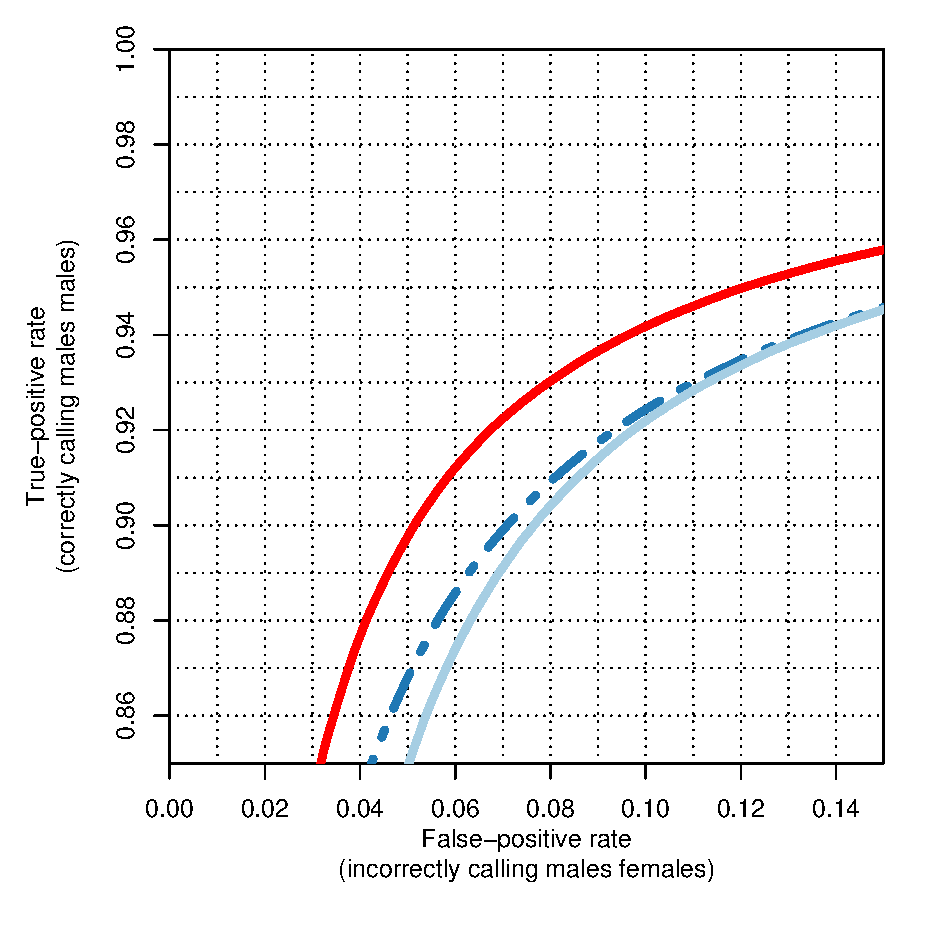
\includegraphics{CRMAv2,chrX,all,ROC,d=0_15}}
 \resizebox{0.49\columnwidth}{!}{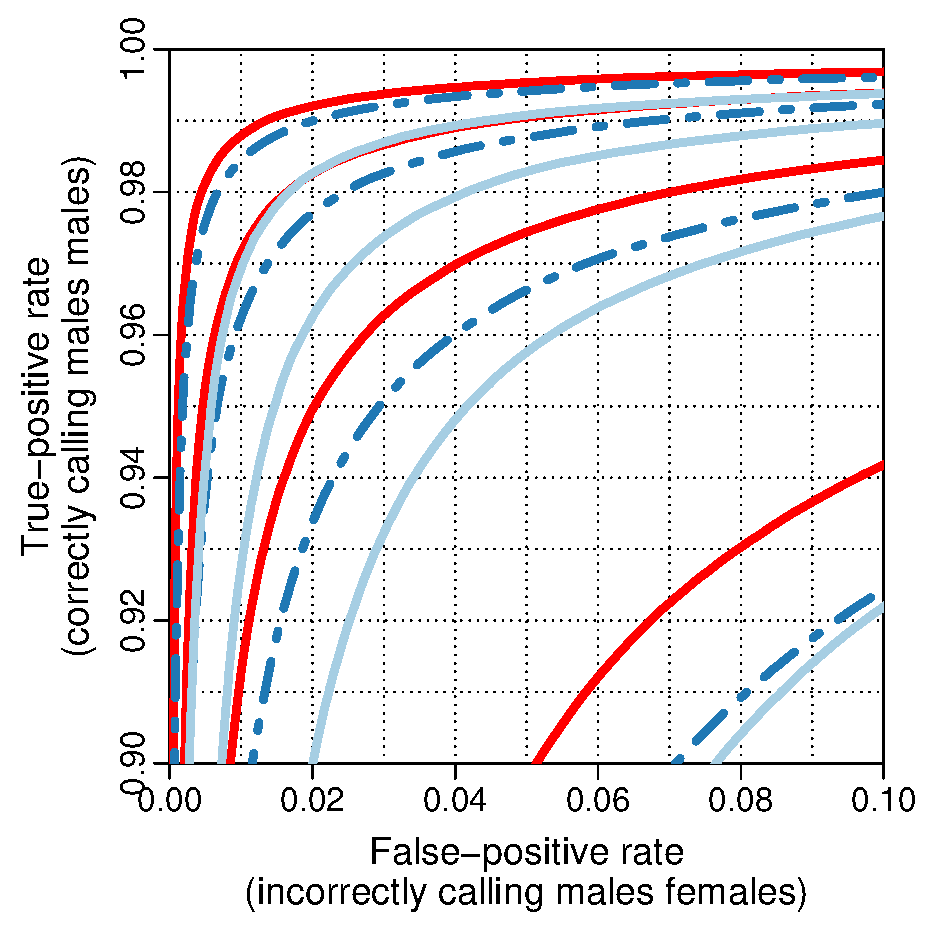
\includegraphics{CRMAv2,chrX,all,smooth1-4,ROC,d=0_10}}
\end{center}
 \caption{
   ROC curves showing that CRMA~v2 (solid red) separates CN=1 from CN=2 (ChrX) better than CN5 (dashed blue) and dChip* (solid light blue) at the full resolution ($H=1$; left panel) as well as at various amounts of smoothing ($H=1,2,3,4$; right panel).  The curves for $H=1$ are in the lower right corner and the curves for $H=4$ are in the upper left corner.
 }
 \label{figRocChrX}
\end{figure}

Using a windowing technique similar to that in~\citet{BengtssonH_etal_2008}, for a fixed \FPrate we can estimate the \TPrate as a function of amount of smoothing.  Since a given amount of smoothing corresponds to a given distance between loci this provides us with a first approximation to the effective resolution of a method.  In the upper panel of Figure~\ref{figTPvResolutionChrXY} the \TPrate (for CN=2 v. CN=1) as a function of resolution is shown for the three methods, which shows that CRMA~v2 has a higher resolution.
\begin{figure}[!tpbh]
\begin{center}
  \resizebox{0.68\columnwidth}{!}{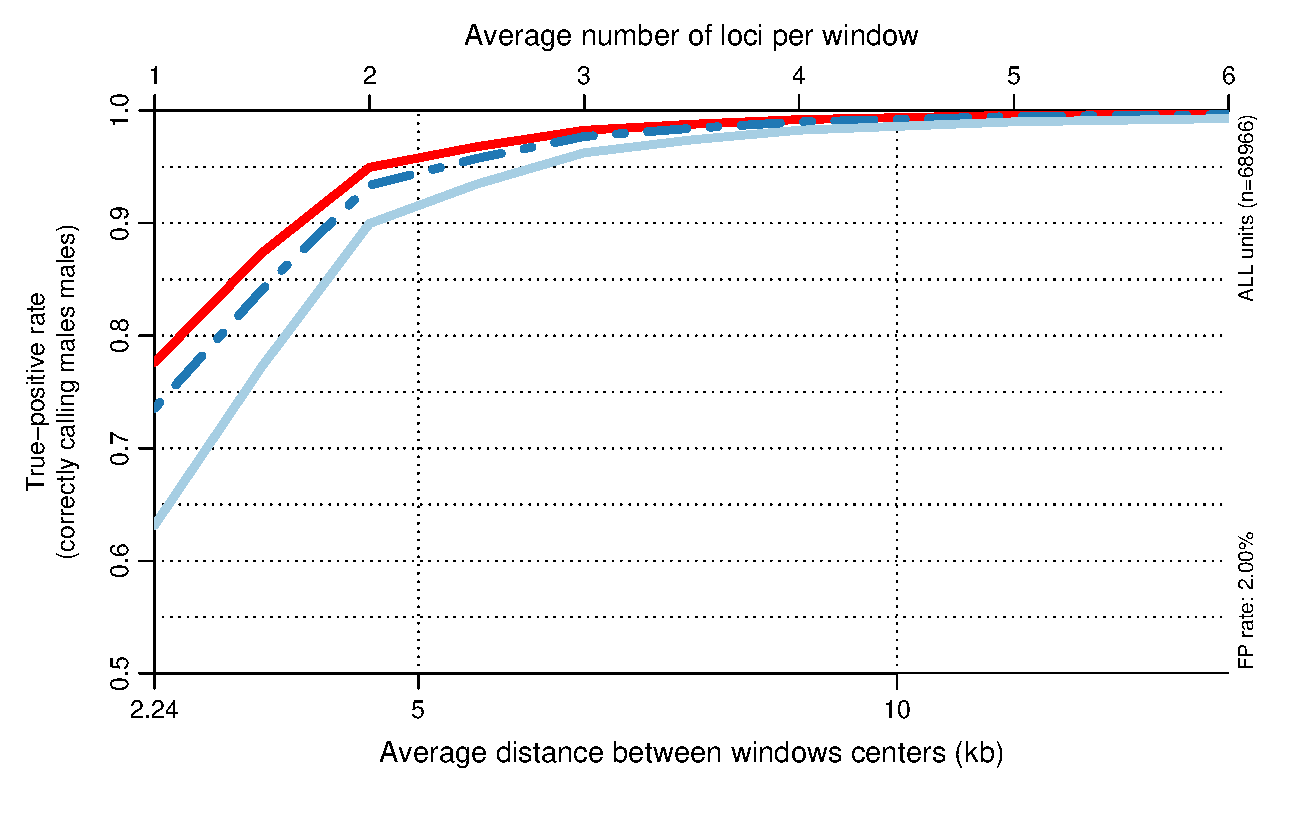
\includegraphics{CRMAv2,chrX,all,tpResolution,fpRate=2_00,y=0_50-1_00}} \\
  \resizebox{0.68\columnwidth}{!}{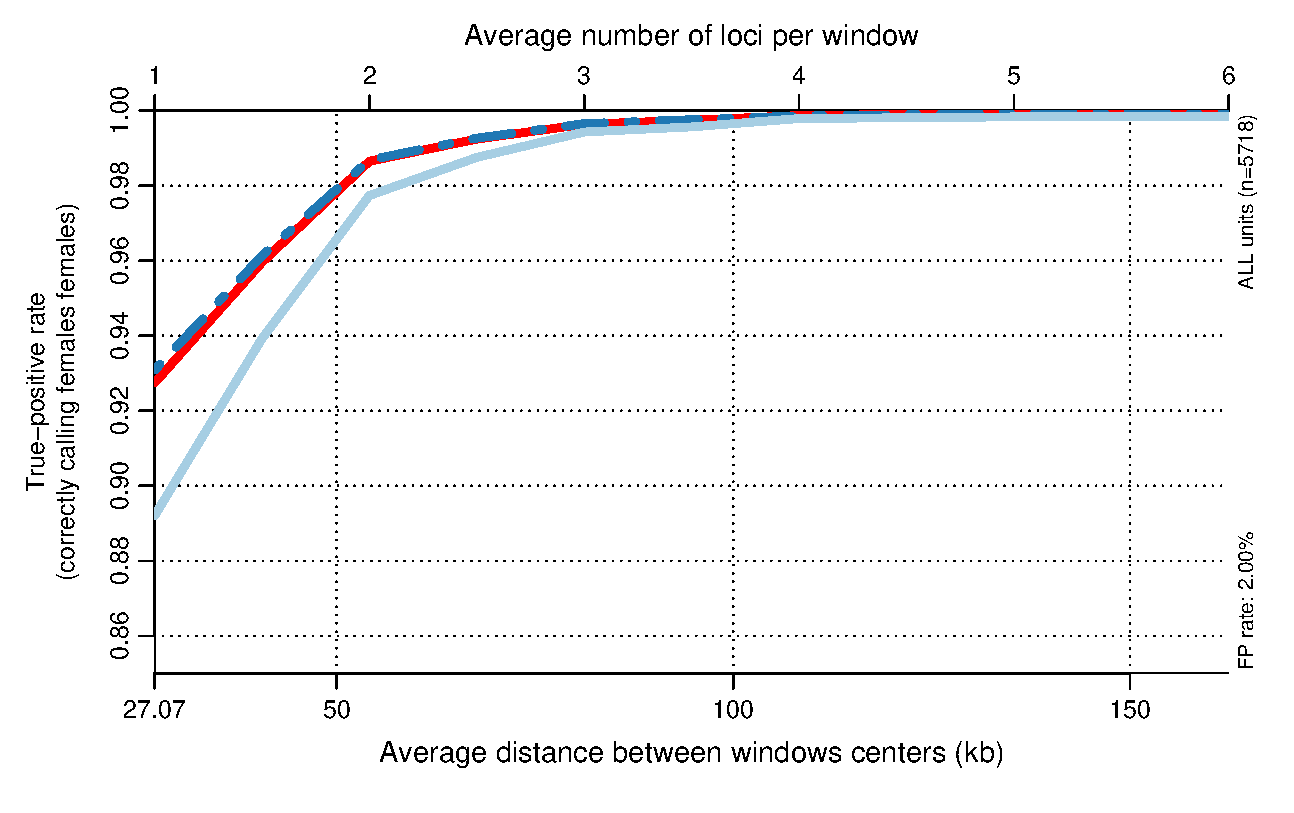
\includegraphics{CRMAv2,chrY,all,tpResolution,fpRate=2_00,y=0_85-1_00}}
\end{center}
 \caption{
   The \TPrate as a function of resolution/smoothing at a 2.0\% \FPrate for the different methods.
   The results for the CN=2 v. CN=1 (ChrX) test is depicted in the upper panel
   and the results for the CN=1 v. CN=0 (ChrY) test in the lower panel.
   Note the different scales.  See Figure~\ref{figRocChrX} for legends.
 }
 \label{figTPvResolutionChrXY}
\end{figure}




\subsubsection{Differentiating CN=0 and CN=1 (ChrY)}
Identifying a CN=0 locus among CN=1 loci is easier than identifying a CN=1 locus among CN=2 loci.  
%% The rationale for this is that the distance between CN=0 and CN=1 is smaller than between CN=1 and CN=2 relative to the reference level.  
This is because the distance between CN=0 and CN=1 is greater than that between CN=1 and CN=2, relative to the reference level (and noise level). 
This is also confirmed by comparing the corresponding \TPrates at a given \FPrate (Figure~\ref{figRocChrX} and Figure~\ref{figRocChrY}) at the full resolution or at various amounts of smoothing (Figure~\ref{figTPvResolutionChrXY}).  
The results also show that CN5 is \updated{as good as}{REMOVED: equally good: ADDED:} or slightly better than CRMA~v2 at differentiating CN=0 from CN=1, and both are better than dChip*.
\updated{In this ROC analysis, which is based on 5,718 loci in 59 samples, there were in total 150,162 CN=0 (female) loci out of 305,502 loci.}{ADDED:}

\begin{figure}[!tpbh]
\begin{center}
 \resizebox{0.49\columnwidth}{!}{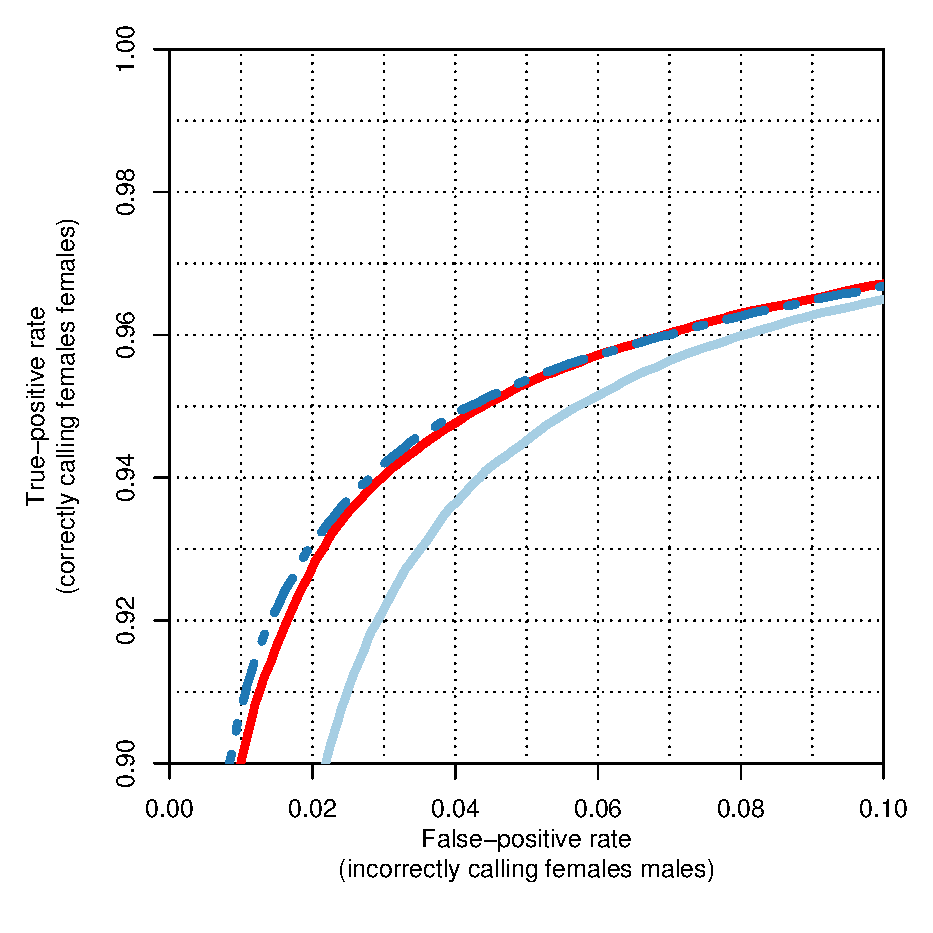
\includegraphics{CRMAv2,chrY,all,ROC,d=0_10}}
 \resizebox{0.49\columnwidth}{!}{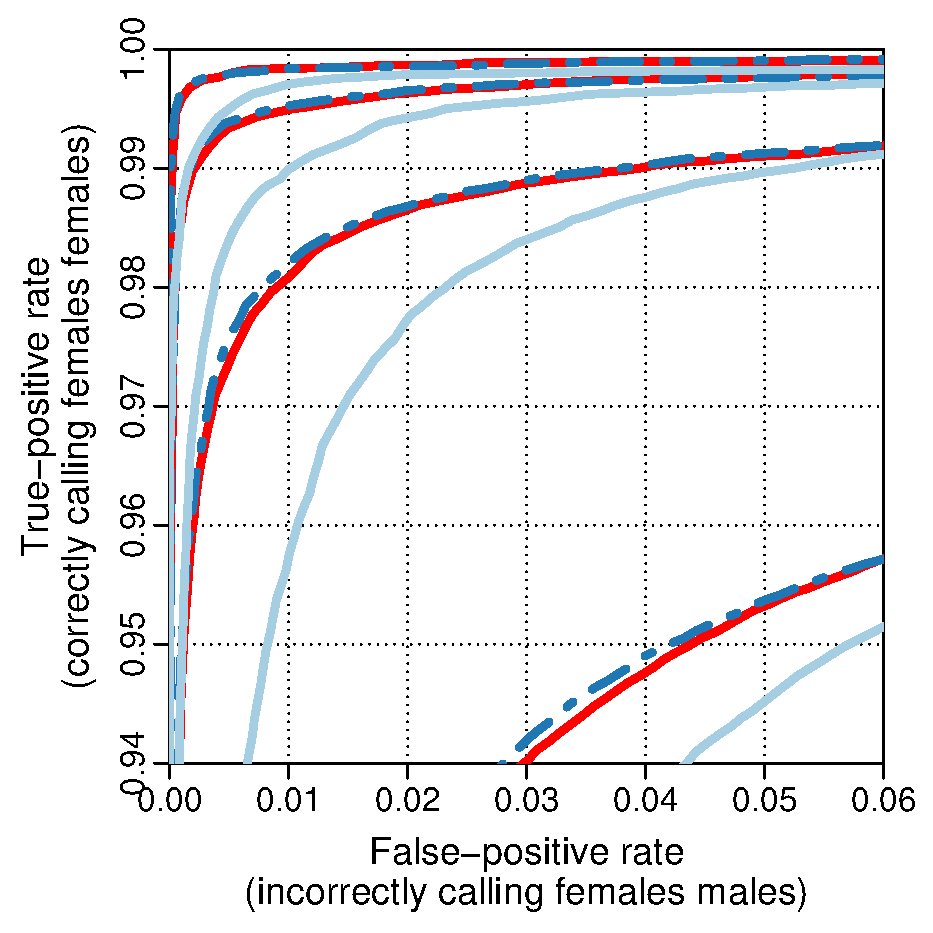
\includegraphics{CRMAv2,chrY,all,smooth1-4,ROC,d=0_06}}
\end{center}
 \caption{
   ROC curves showing CRMA~v2 differentiates between CN=1 and CN=0 (ChrY) as good as or slightly worse than CN5, and better than dChip* at the full resolution (left panel) as well as at various amounts of smoothing (right panel).  
   See Figure~\ref{figRocChrX} for legends.
 }
 \label{figRocChrY}
\end{figure}



\subsubsection{Performance of SNPs and CN loci}
In order to better understand differences between methods, we compare the ROC curves and distribution of \TPrates at a given \FPrate~\citep{BengtssonH_etal_2008} while stratifying on SNP and CN loci.
We observe that on average the discriminatory power is greater for SNPs than CN loci (upper panels of Figure~\ref{figROC-SNPvCNChrX} and Figure~\ref{figROC-SNPvCNChrY}).  CN5 is the method for which SNPs and CN loci have the most similar performances.   Furthermore, by investigating the locus-by-locus ROCs, we observe that the \TPrates at a fixed \FPrate tend to be greater for SNPs than for CN loci (lower panels), and that there is a significant set of CN loci with very low \TPrates.  The dChip* method has a larger set of poorly performing CN loci, which is also seen when comparing dChip's ROC curves for SNPs and CN loci.  
\updated{For the ChrX-based analysis 30,238 SNPs and 38,728 CN loci were used, and for the ChrY-based analysis 208 SNPs and 5,510 CN loci were used.}{ADDED:}

\begin{figure}[!tpbh]
\begin{center}
 \begin{tabular}{cc}
 \resizebox{0.49\columnwidth}{!}{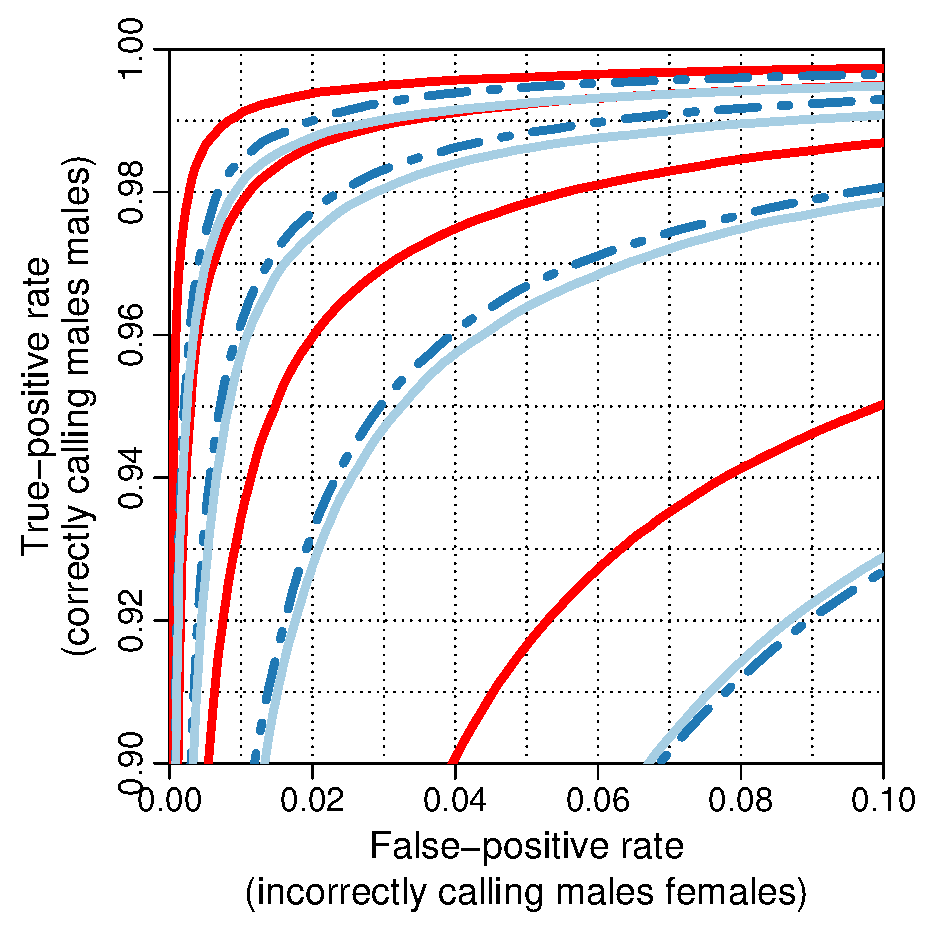
\includegraphics{CRMAv2,chrX,snp,smooth1-4,ROC,d=0_10}} &
 \resizebox{0.49\columnwidth}{!}{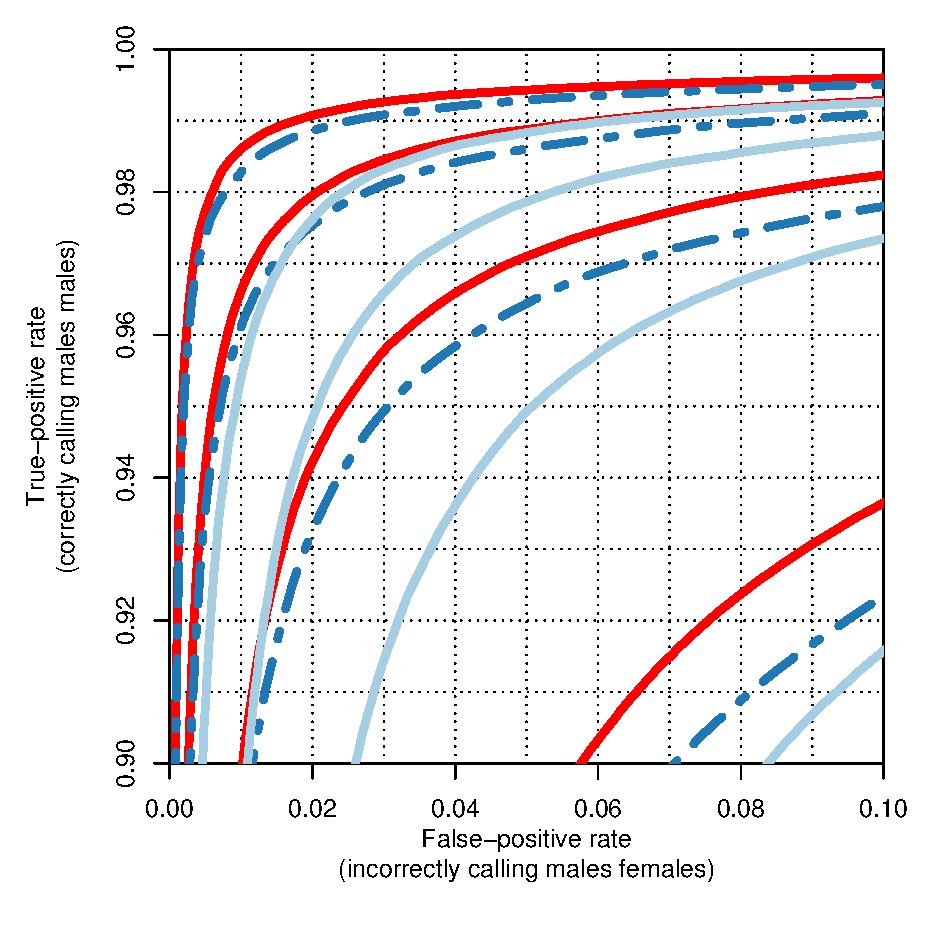
\includegraphics{CRMAv2,chrX,cn,smooth1-4,ROC,d=0_10}} \\
 \resizebox{0.49\columnwidth}{!}{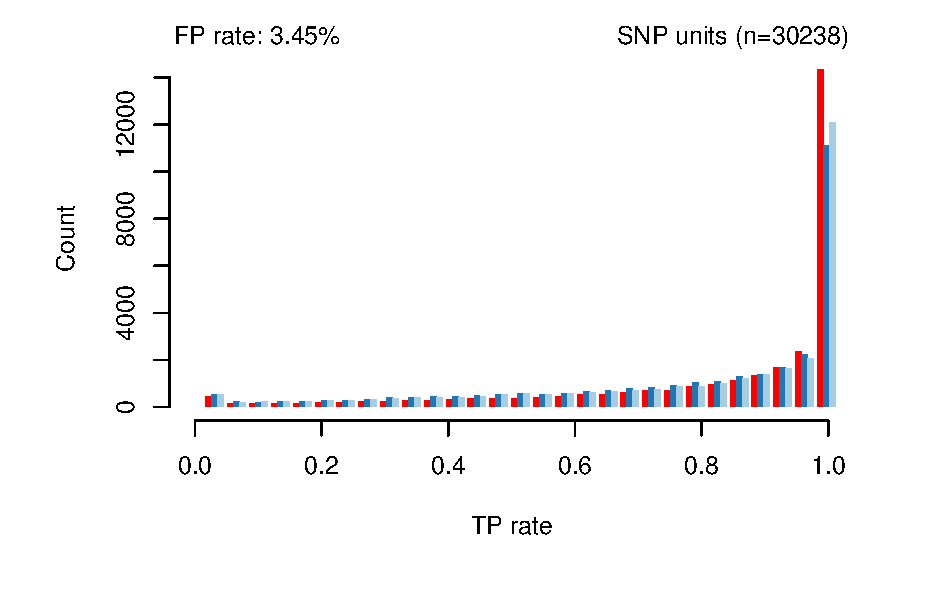
\includegraphics[bb=16 16 402 265,clip=true]{CRMAv2,chrX,snp,tpHist,fpRate=3_45}} &
 \resizebox{0.49\columnwidth}{!}{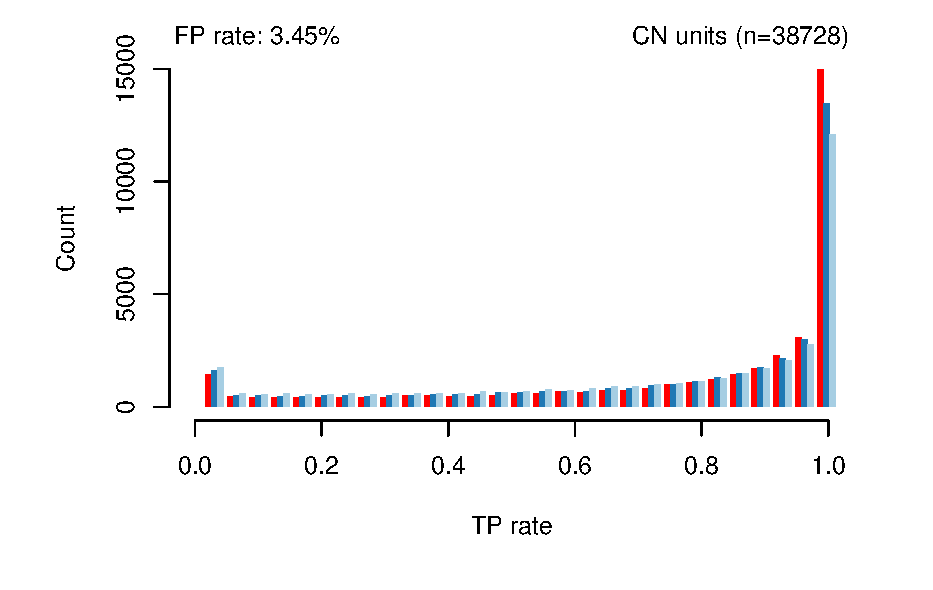
\includegraphics[bb=16 16 402 265,clip=true]{CRMAv2,chrX,cn,tpHist,fpRate=3_45}}
 \end{tabular}
\end{center}
 \caption{
  Performance on SNPs (left) and CN units (right) for CRMA~v2 (solid red; left bars), CN5 (dashed blue; middle bars) and dChip* (solid light blue; right bars) when testing for CN=2 v. CN=1 (ChrX).
  The upper panels show the ROC curves for $H=1,2,3,4$ and the lower panels show the distribution of \TPrates at fixed \FPrate (1.72\%).
 }
 \label{figROC-SNPvCNChrX}
\end{figure} 


\begin{figure}[!tpbh]
\begin{center}
 \begin{tabular}{cc}
 \resizebox{0.49\columnwidth}{!}{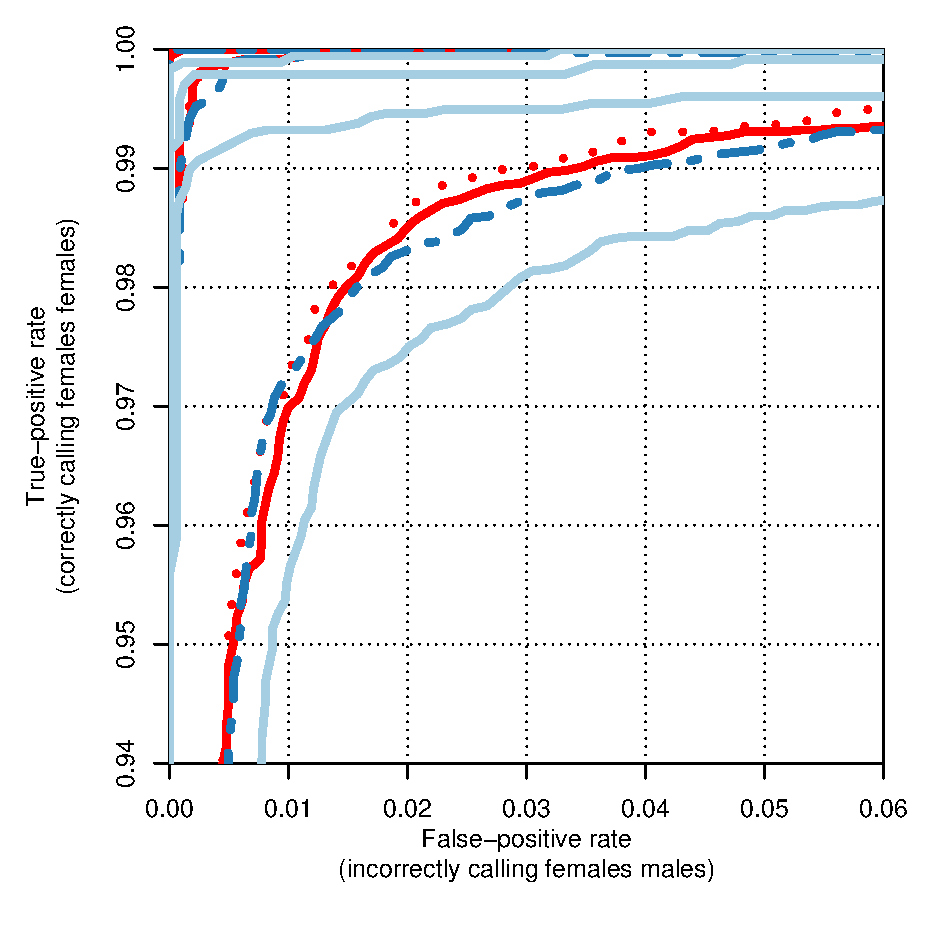
\includegraphics{CRMAv2,chrY,snp,smooth1-4,ROC,d=0_06}} &
 \resizebox{0.49\columnwidth}{!}{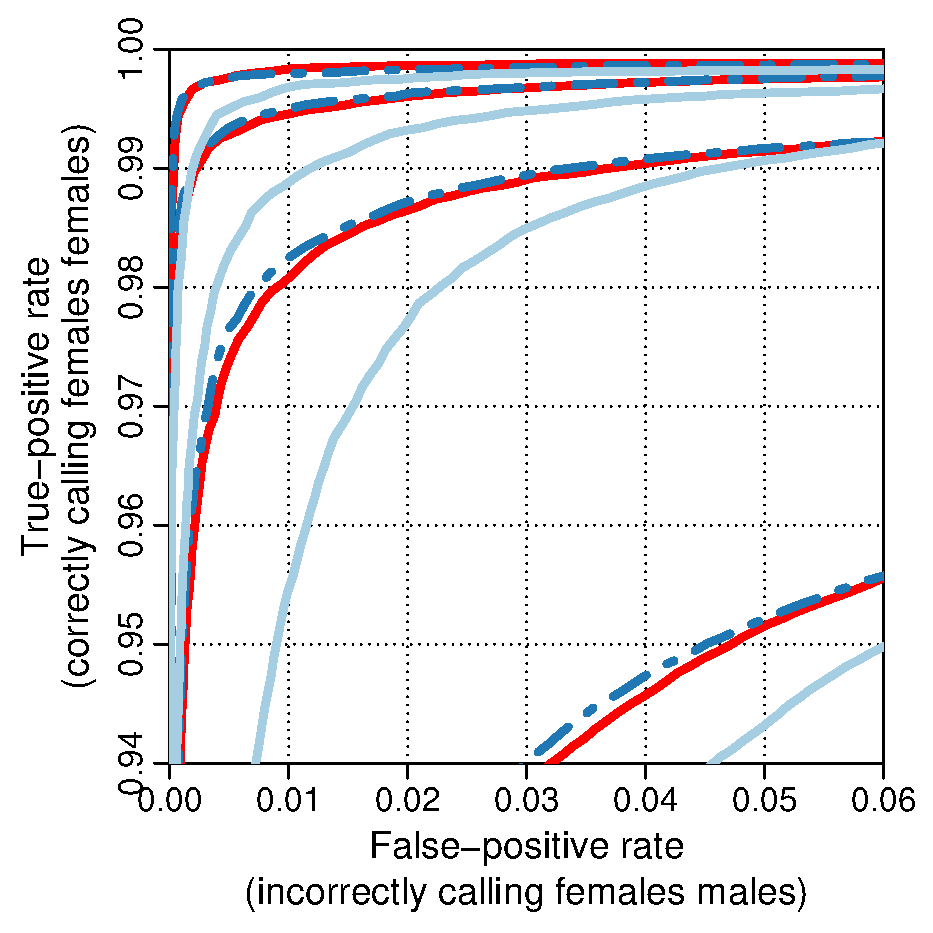
\includegraphics{CRMAv2,chrY,cn,smooth1-4,ROC,d=0_06}} \\
 \resizebox{0.49\columnwidth}{!}{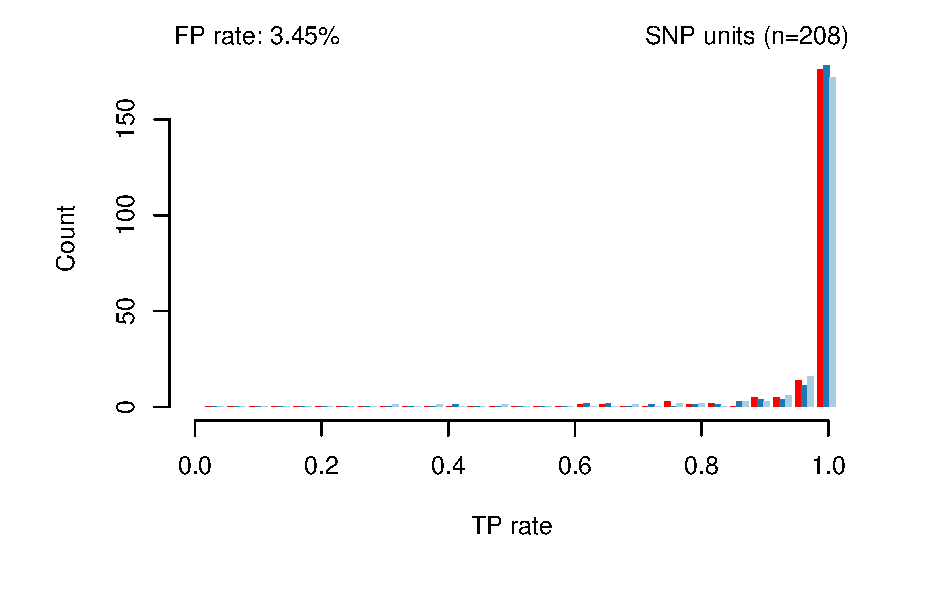
\includegraphics[bb=16 16 402 265,clip=true]{CRMAv2,chrY,snp,tpHist,fpRate=3_45}} &
 \resizebox{0.49\columnwidth}{!}{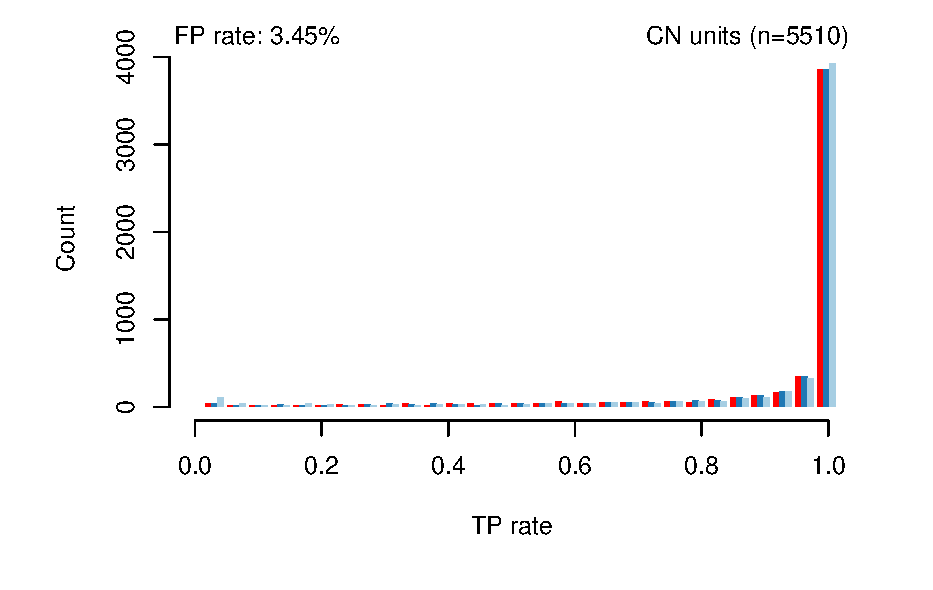
\includegraphics[bb=16 16 402 265,clip=true]{CRMAv2,chrY,cn,tpHist,fpRate=3_45}}
 \end{tabular}
\end{center}
 \caption{
  Performance on SNPs (left) and CN units (right) for CRMA~v2, CN5 and dChip* when testing for CN=1 v. CN=0 (ChrY).
  The upper panels show the ROC curves for $H=1,2,3,4$ and the lower panels show the distribution of \TPrates at fixed \FPrate (1.72\%).
  Legends as in Figure~\ref{figROC-SNPvCNChrX}.
 }
 \label{figROC-SNPvCNChrY}
\end{figure} 


\subsection{Single-sample evaluation}
\label{secSingleSampleEvaluation}
\updated{For the tumor-normal pair HCC1143, we calculated how well CN estimates of loci that are either gains or losses separate from estimates of copy-neutral loci.  Figures~\ref{figROC-GSM337641,Chr01} and \ref{figROC-GSM337641,Chr10} show the CN estimates and the performance for a 7.4Mb region on Chr~1 and 9.0Mb region on Chr~10, respectively.  The former contains a loss (2,074 out of 4,316 loci) and the latter a gain (2,805 out of 5,285 loci).  The ROC results show that CRMA~v2 identifies the aberrant states better than or as good as dChip* and CN5.  We wish to emphasize that in order for CRMA~v2 to provide CN estimates for this tumor-normal pair only two CEL files were required.  For dChip* and CN5 all 68 CEL files were used in order to obtain CN estimates.  Results for additional CN regions and amounts of smoothing can found in the Supplementary Notes.
}{ADDED:}
\begin{figure}[!tpbh]
\begin{center}
 \resizebox{0.96\columnwidth}{!}{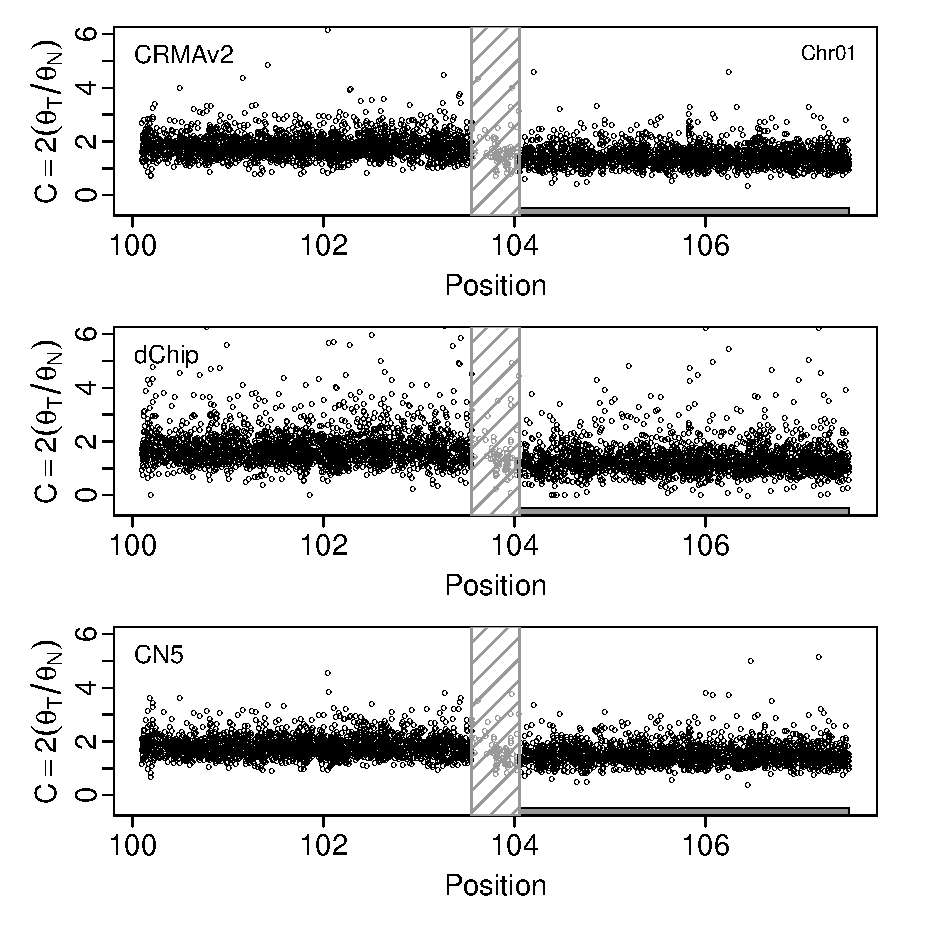
\includegraphics{GSM337641,chr01,100_1-107_5,ratios,track}} \\
 \resizebox{\columnwidth}{!}{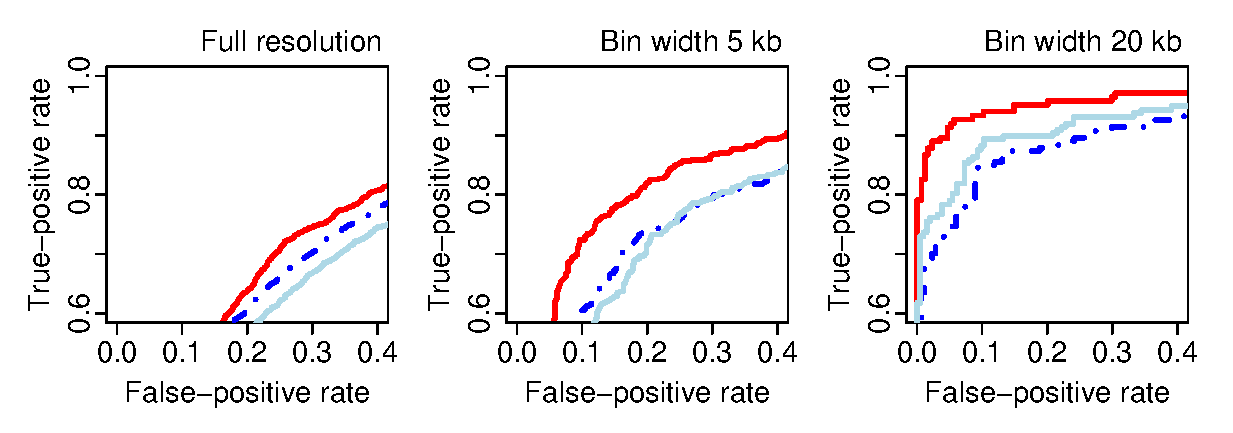
\includegraphics{GSM337641,chr01,100_1-107_5,ratios,ROC}} \\
\end{center}
 \caption{
  The region 100.1-107.5Mb on Chr~1 in tumor-normal sample HCC1143 has a change points at approximately 103.8Mb, which separates a copy-neutral state (left) from a loss (right).
  There are 2,242 and 2,074 loci in these two states, respectively (totaling 4,316 loci).
  The top three rows show the raw CNs (Eqn~\eqref{eqnCnRatio}) of the CRMA~v2, the dChip, and the CN5 methods, respectively.  The 500kb safety region around the change point with data points excluded in the evaluation is highlighted by a dashed frame.  The three panels in the bottom row shows the ROC performance of the three methods at the full resolution, and after binning the CNs in non-overlapping windows of size 5kb and 20kb, respectively.
  Legends as in Figure~\ref{figROC-SNPvCNChrX}.
 }
 \label{figROC-GSM337641,Chr01}
\end{figure} 

\begin{figure}[!tpbh]
\begin{center}
 \resizebox{0.96\columnwidth}{!}{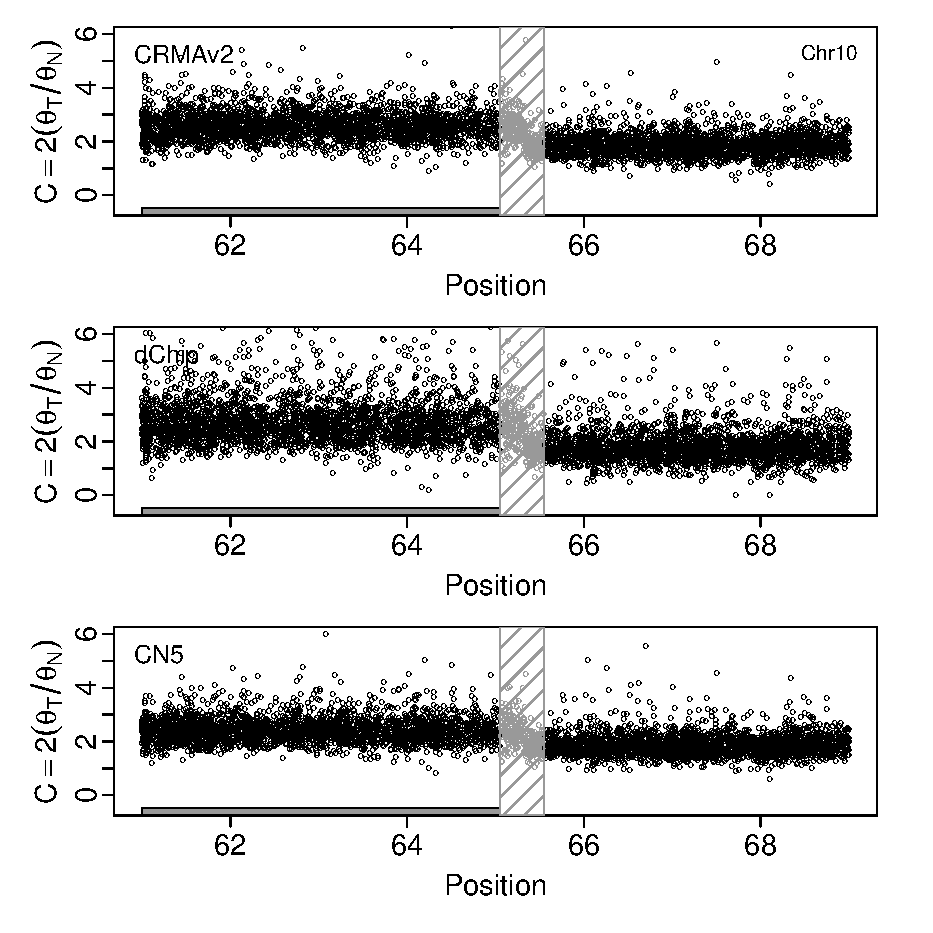
\includegraphics{GSM337641,chr10,61-69,ratios,track}} \\
 \resizebox{\columnwidth}{!}{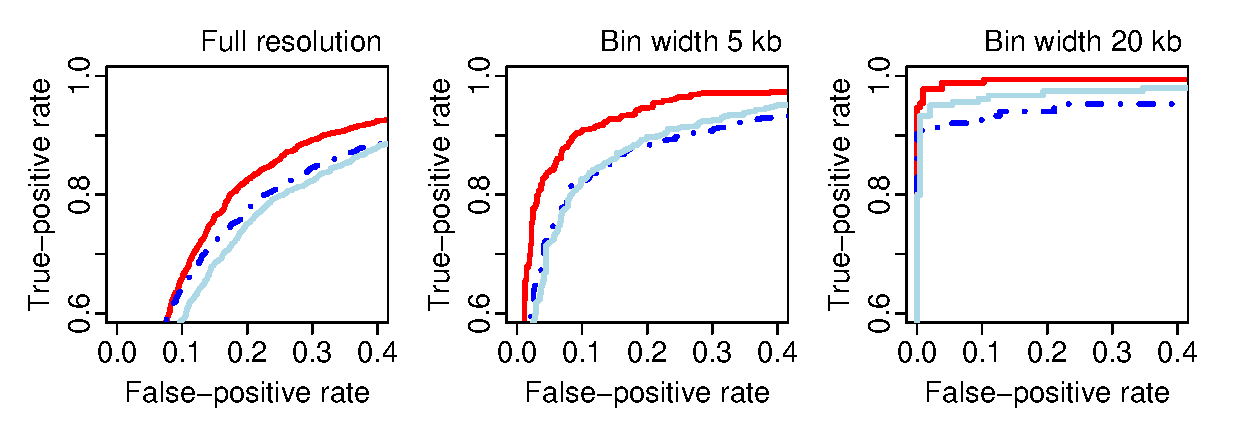
\includegraphics{GSM337641,chr10,61-69,ratios,ROC}} \\
\end{center}
 \caption{
  The region 61.0-69.0Mb on Chr~10 in tumor-normal sample HCC1143 has a change points at approximately 65.3Mb, which separates a gain (left) from a copy-neutral state (right).  There are 2,805 and 2,480 loci in these two states, respectively (totaling 5,285 loci).
  Content and legends as in Figure~\ref{figROC-GSM337641,Chr01}.
 }
 \label{figROC-GSM337641,Chr10}
\end{figure} 


%%%%%%%%%%%%%%%%%%%%%%
\section{Discussion}
\label{secDiscussion}
We conclude that it is possible for a single-array method such as CRMA~v2 to produce non-polymorphic CN estimates that discriminate two CN states \updated{as good as}{REMOVED: equally well: ADDED:} or better than existing multi-array based methods.
%% With a single-array method each array can be processed independently of the others.  This have several implications.  Each array can be preprocessed immediately after being scanned.  Arrays can be processed in parallel on different hosts making it possible to decrease the processing time of a set of arrays linearly with the number of hosts.  There is no need to reprocess an array when new arrays are produced, which further saves time and computational resources.  
%% Moreover, this is potentially very practical for applied medical diagnostics, because individual patients can be analyzed even when they come in trickles (instead of in batches).
%%Furthermore, the decision to filter out poor samples can be made later, because a poor sample will not affect the estimates of other arrays, which is illustrated by the exclusion of sample NA12145 in this study.
Our study confirms that it is harder to differentiate between CN=1 and CN=2 than between CN=0 and CN=1.  We believe that this trend will be true for higher CN levels, i.e. it will be harder and harder to separate higher CN levels from each other.
%%
We also found that the SNPs show stronger discrimination for copy number than the CN loci.
%% We also found that SNPs have more power [HB: are these correct words to use?] than CN loci. 
We look forward to further studies investigating whether this is because more/multiple probes are used for the SNPs or there are other reasons for this.
\updated{Also, an assessment is still needed of}{REMOVED: Also, it still has to be assessed ADDED:} how well CRMA~v2 (and other methods) controls for systematic effects between labs and batches, and whether additional normalization is needed in such cases.

We also wish to emphasize that the dChip method has not been optimized for \GWS or SNP arrays, which may explain its lower performance in this \GWSSix study in comparison with its higher performance for the 500K arrays~\citep{BengtssonH_etal_2008}.


%% The sex-chromosome evaluation method used favors methods that produce CN estimates that have consistent mean CN levels across samples.  Hence, a method that produces estimates with great discrepancy power per array but does not control for the mean levels across arrays will be penalized.  This might be one reason why CRMA~v2 performs better than the other methods.  An alternative is to identify known CN aberrations within each sample, assume that the CNs are constant within each such region, and then test how well each method can separate between the CN level inside and outside each region.  Such an evaluation will not penalize against differences between arrays, but only focus on within array performances.  Which kind of evaluation method to use, depends on what the main objective is.

CRMA~v2 provides neither allele-specific nor \updated{CN estimates calibrated toward true CN levels.}{DELETE: calibrated CN estimates. ADDED:}  Allele-specific CNs are needed in order to identify events such as copy-neutral loss-of-heterozygosity (LOH).  With calibrated allele-specific CNs, genotyping algorithms can be generalized to call genotypes beyond the traditional diploid AA, AB, and BB states.  We are currently working on an extension to CRMA~v2 that will provide full-resolution calibrated allele-specific CN estimates.

  

    
%%%%%%%%%%%%%%%%%%%%%%%%%%%%%%%%
%\section*{Authors contributions}
%HB proposed the model and conducted the analysis.

    

%%%%%%%%%%%%%%%%%%%%%%%%%%%
\section*{Acknowledgements}
We wish to thank Ben Bolstad, Simon Cawley, and Jim Veitch at Affymetrix Inc. for technical support and scientific feedback.
We also thank Cheng Li at the Harvard School of Public Health for details on the dChip method and software, and the reviewers for constructive feedback.
HB was supported by grants from the Wenner-Gren Foundation, the American-Scandinavian Foundation, and the Solander Foundation.\\[1ex]



\bibliography{bioinformatics-journals-abbr,hb-at-maths.lth.se}
\bibliographystyle{natbib}
 
%\begin{thebibliography}{}
%\end{thebibliography} 

\clearpage
\section*{Updates to this manuscript}
\theendnotes

\end{document}

%%%%%%%%%%%%%%%%%%%%%%%%%%%%%%%%%%%%%%%%%%%%%%%%%%%%%%%%%%%%%%%%%%%%%%
% 2009-04-06 [HB]
% o Began to enter the updates for the revision.
% 2009-01-05
% o Received reviews.
% 2008-11-04
% o Submitted to Oxford Bioinformatics.
%%%%%%%%%%%%%%%%%%%%%%%%%%%%%%%%%%%%%%%%%%%%%%%%%%%%%%%%%%%%%%%%%%%%%%
